
\section*{Preliminary results}

A sample of 800,000 events was generated following the prescription above. Proton-proton collisions leading to a single vector leptoquark with final states involving a $b$-quark and $\tau$ lepton were considered. The MadGraph input for generating these events is as follows:
\begin{verbatim}
    import model Mod2_VLQ_UFO
    define p = g u c d s u~ c~ d~ s~ b b~
    define j = g u c d s u~ c~ d~ s~
    define ta = ta+ ta-
    define qb = b b~
    define lq = vlq vlq~
    generate p p > j ta lq, lq > ta qb
    output Single_LQ/Single_vlq_mlq500 -nojpeg
\end{verbatim}

The simulations demand fixing the values of all model constants. The leptoquark mass was arbitrarily fixed at $500\;\si{GeV}$. Further study may involve different masses for the leptoquark. The model's coupling constants were chosen with high regard towards experimental constraints. The choice (see table \ref{tab:parameters}) was made according to \cite{cornella_reading_2021}, where coupling constants in different scenarios were chosen to fit the data. From the scenarios, the one with maximal right-handed currents was chosen in order to enhance the branching ratio to leptoquarks, with the further assumption of minimal $U(2)^5$ flavour symmetry breaking, since this assumption was already made in the UFO model.

\begin{table}[ht]
    \centering
    \begin{tabular}{c|c}
        \toprule
        Parameter & Value \\ \midrule
        $g_U$ & 0.29 \\
        $\beta_R^{ij}$ & 0 (if $i,j<3$ and $i\neq j$)\\
        $\beta_R^{b\tau}$ & -1 \\
        $\beta_L^{b\tau}$ & 1 \\
        $\beta_L^{b\mu}$ & -0.21 \\
        $\beta_L^{s\tau}$ & 0.21 \\
        $\beta_L^{s\mu}$ & 0.03 \\ \bottomrule
    \end{tabular}
    \caption{Values of model parameters used in the simulations. These values are the best fit to experimental observations as reported in \cite{cornella_reading_2021}}
    \label{tab:parameters}
\end{table}

The dominant diagrams for the generated processes are shown in figure \ref{fig:dominant}. Among these, the analysis was focused towards those that exhibit a VBF-like topology, as shown in fig. \ref{fig:feynman-VBFlike}. For diagrams of this type, event detection at the CMS involves the hadronisation and/or leptonic decay of the final states. In this case, event selection was devoted to thethe semi-leptonic channel were selected; that is when one of the $\tau$'s decays via a weak boson into a lepton-neutrino pair and the other decays hadronically. The semi-leptonic channel was treated as two sub-channels: with the $\tau$ decaying into electron-neutrino and muon-neutrino pairs. The event selection involved a series of cuts, which are summarised in table \ref{tab:cuts}. The code implementing these cuts is available on \href{https://github.com/DanielDoradoPhys/LeptoquarksPheno}{GitHub}.

\begin{table}[ht]
    \centering
    \begin{tabular}{l|c c c |c c c }
        \toprule
        & \multicolumn{3}{c}{$\tau \to e\nu$} & \multicolumn{3}{c}{$\tau \to \mu\nu$}  \\ 
        & Events & Abs. eff. & Rel. eff. & Events & Abs. effi. & Rel. eff. \\\midrule
        All events & 800000 & $100.00\%$ &  $100.00\%$ & 800000 & $100.00\%$ &  $100.00\%$ \\
        More than two jets & 783618 & $97.95\%$ & $97.95\%$ & 783618 & $97.95\%$ & $97.95\%$ \\
        One useful lepton & 131630 & $16.45\%$ & $16.79\%$ & 153540 & $19.19\%$ & $19.59\%$ \\
        No leptons of the other type & 116873 & $14.61\%$ & $88.79\%$ & 138770 & $17.34\%$ & $90.38\%$ \\
        At least one $\tau$-jet & 54076 & $6.75\%$ & $46.26\%$ & 64368 & $8.04\%$ & $46.38\%$ \\
        Exactly one $\tau$-jet & 53504 & $6.69\%$ & $98.94\%$ & 63721 & $7.96\%$ & $98.99\%$ \\
        At least one $b$-jet & 39050 & $4.88\%$ & $72.98\%$ & 46496 & $5.81\%$ & $72.96\%$ \\
        Exactly one $b$-jet & 29607 & $3.70\%$ & $75.82\%$ & 35169 & $4.40\%$ & $75.64\%$ \\
        At least one light jet & 28777 & $3.59\%$ & $97.19\%$ & 34228 & $4.28\%$ & $97.32\%$ \\
        \bottomrule
    \end{tabular}
    \caption{Number of events with absolute and relative efficiencies for each condition in the cut. The cuts are shown for both decay modes.}
    \label{tab:cuts}
\end{table}

\begin{figure}
    \centering
    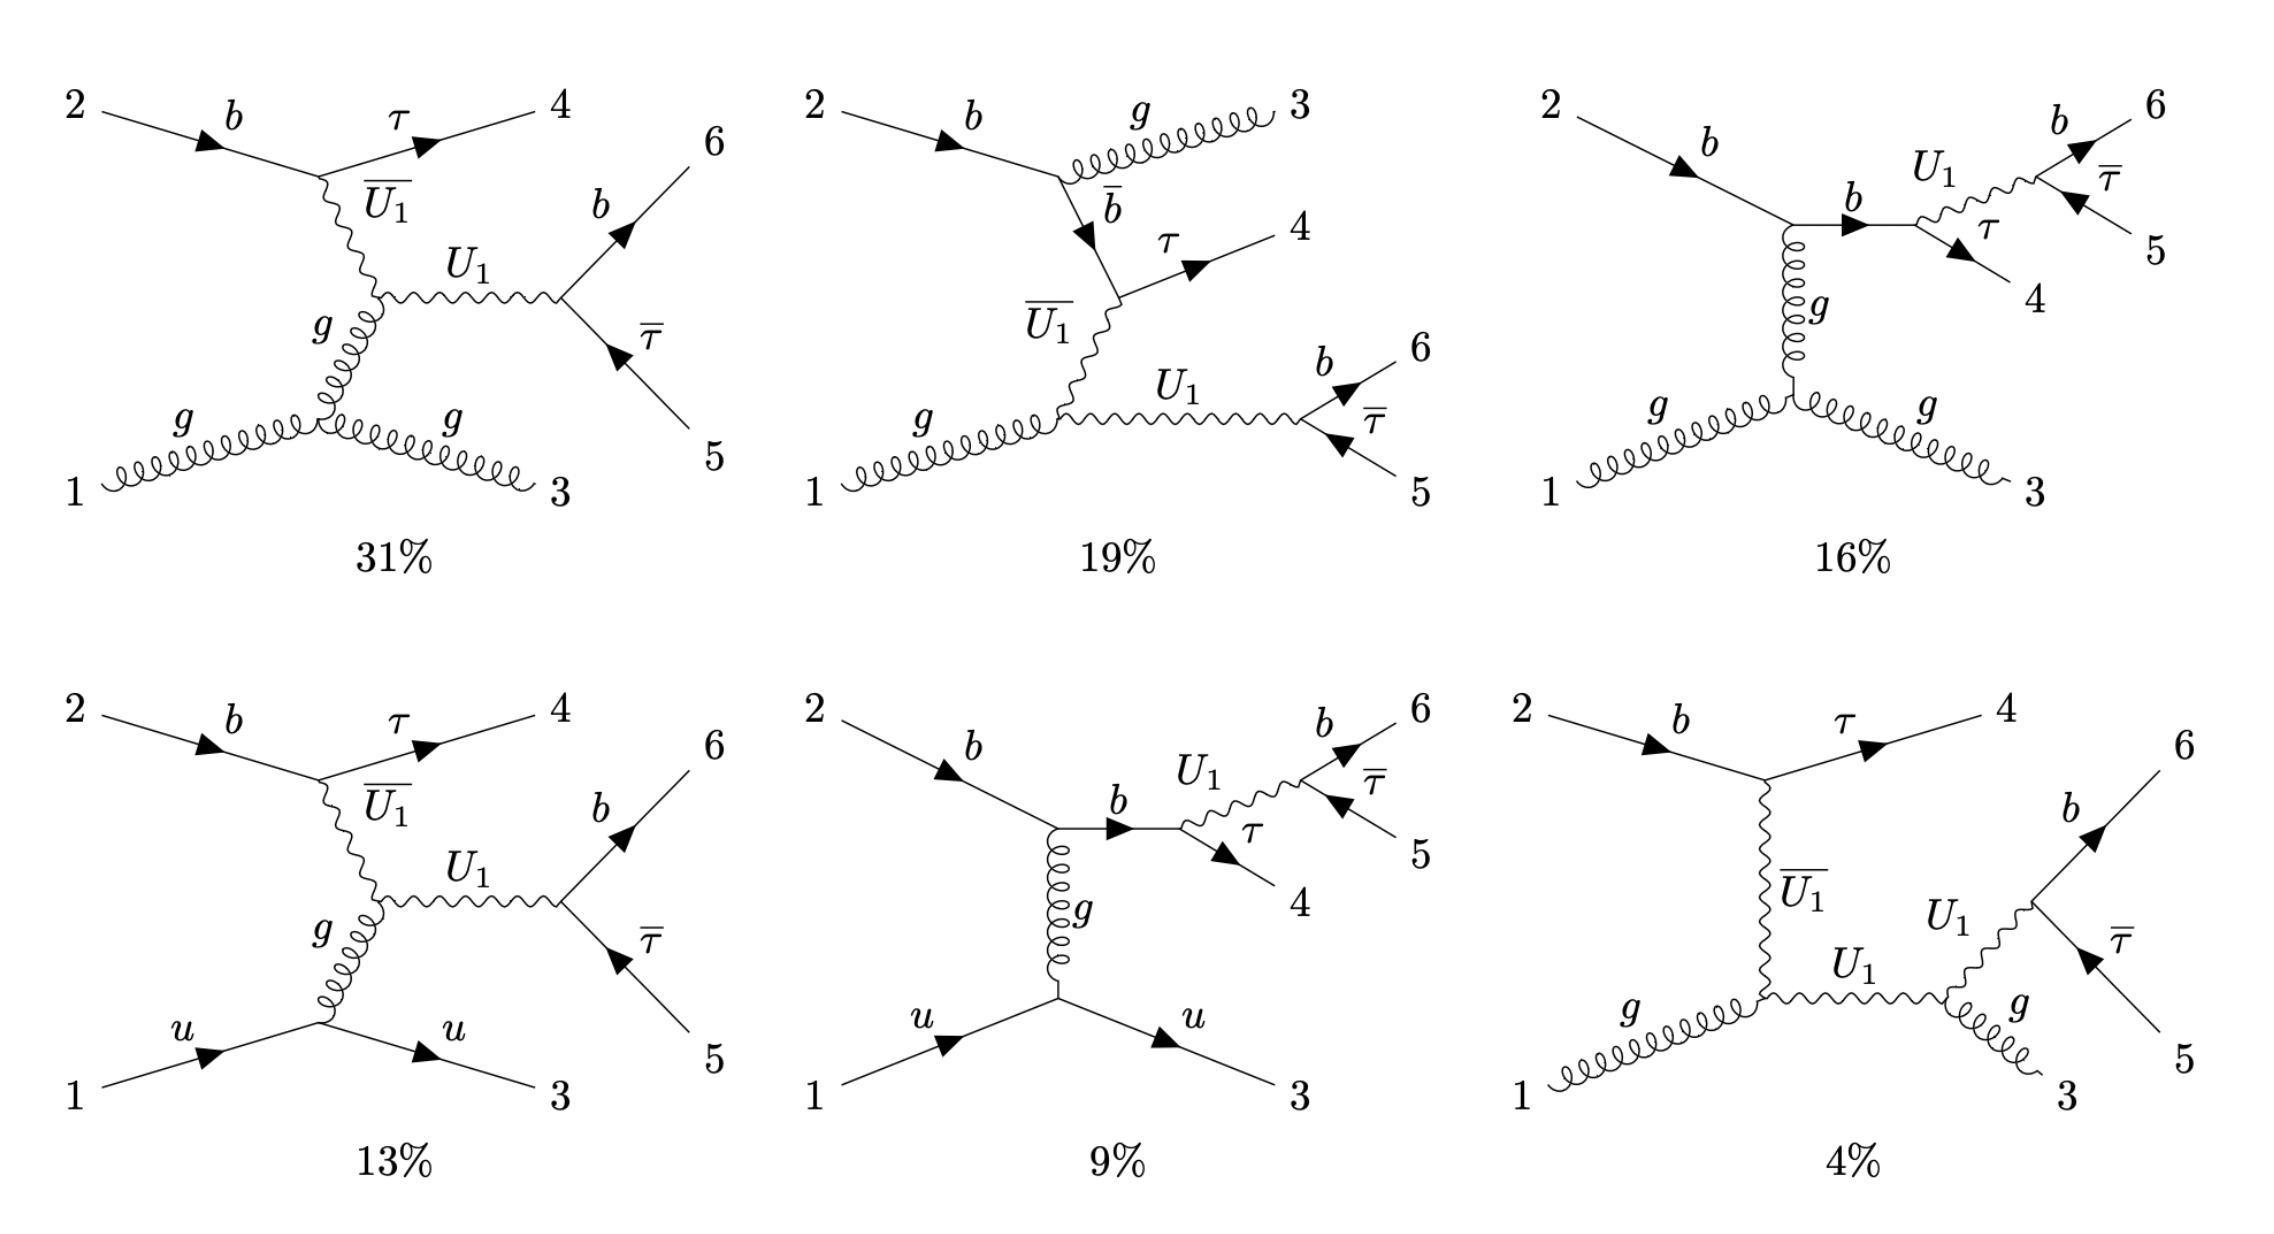
\includegraphics[width=\textwidth]{images/dominant_diagrams.png}
    \caption{Dominant diagrams for the proton-proton collision resulting in a leptoquark which decays into third generation fermions. The total cross-section is $0.067\;\si{pb}$. Below each diagram one can find its contribution to the cross-section.}
    \label{fig:dominant}
\end{figure}

\begin{figure}
    \centering
    \begin{tikzpicture}
      \begin{feynman}
        \vertex (i1) at (-3,2.4) {\(b\)};
        \vertex (i2) at (0,1.5);
        \vertex (i3) at (3,2.4) {\(\tau\)};
        \vertex (a) at (0.75,0);
        \vertex (f1) at (-3,-2.4) {\(j\)};
        \vertex (f2) at (0,-1.5);
        \vertex (f3) at (3,-2.4) {\(j\)};
        \vertex (b) at (3, 0);
        \vertex [above right=of b] (e1) {\(\tau\)};
        \vertex [below right=of b] (e2) {\(b\)};
        
        
        \diagram* {
          (i1) --  (i2) -- (i3),
          (f1) -- (f2) --  (f3),
          (i2) -- [boson, edge label={\(U_1\)}] (a),
          (f2) -- [boson, edge label={\(\gamma, Z, g\)}] (a),
          (a) -- [boson, edge label=\(U_1\)] (b),
          (b) -- (e1),
          (b) -- (e2),
        };
      \end{feynman}
    \end{tikzpicture}
    \caption{Feynman diagram for the VBF-like production of a single leptoquark.}
    \label{fig:feynman-VBFlike}
\end{figure}

After running the event selection, the transverse momentum of the signals was analysed using ROOT. The outcome of this analysis is shown in fig. \ref{fig:pT}. The main takeaway is that the $b$-jet is more energetic than the $\tau$-jet in both subchannels and that the leptons and light-jets seem to have a similar distribution, although leptons are in average less energetic. 

\begin{figure}
    \centering
    \begin{subfigure}{.5\textwidth}
      \centering
      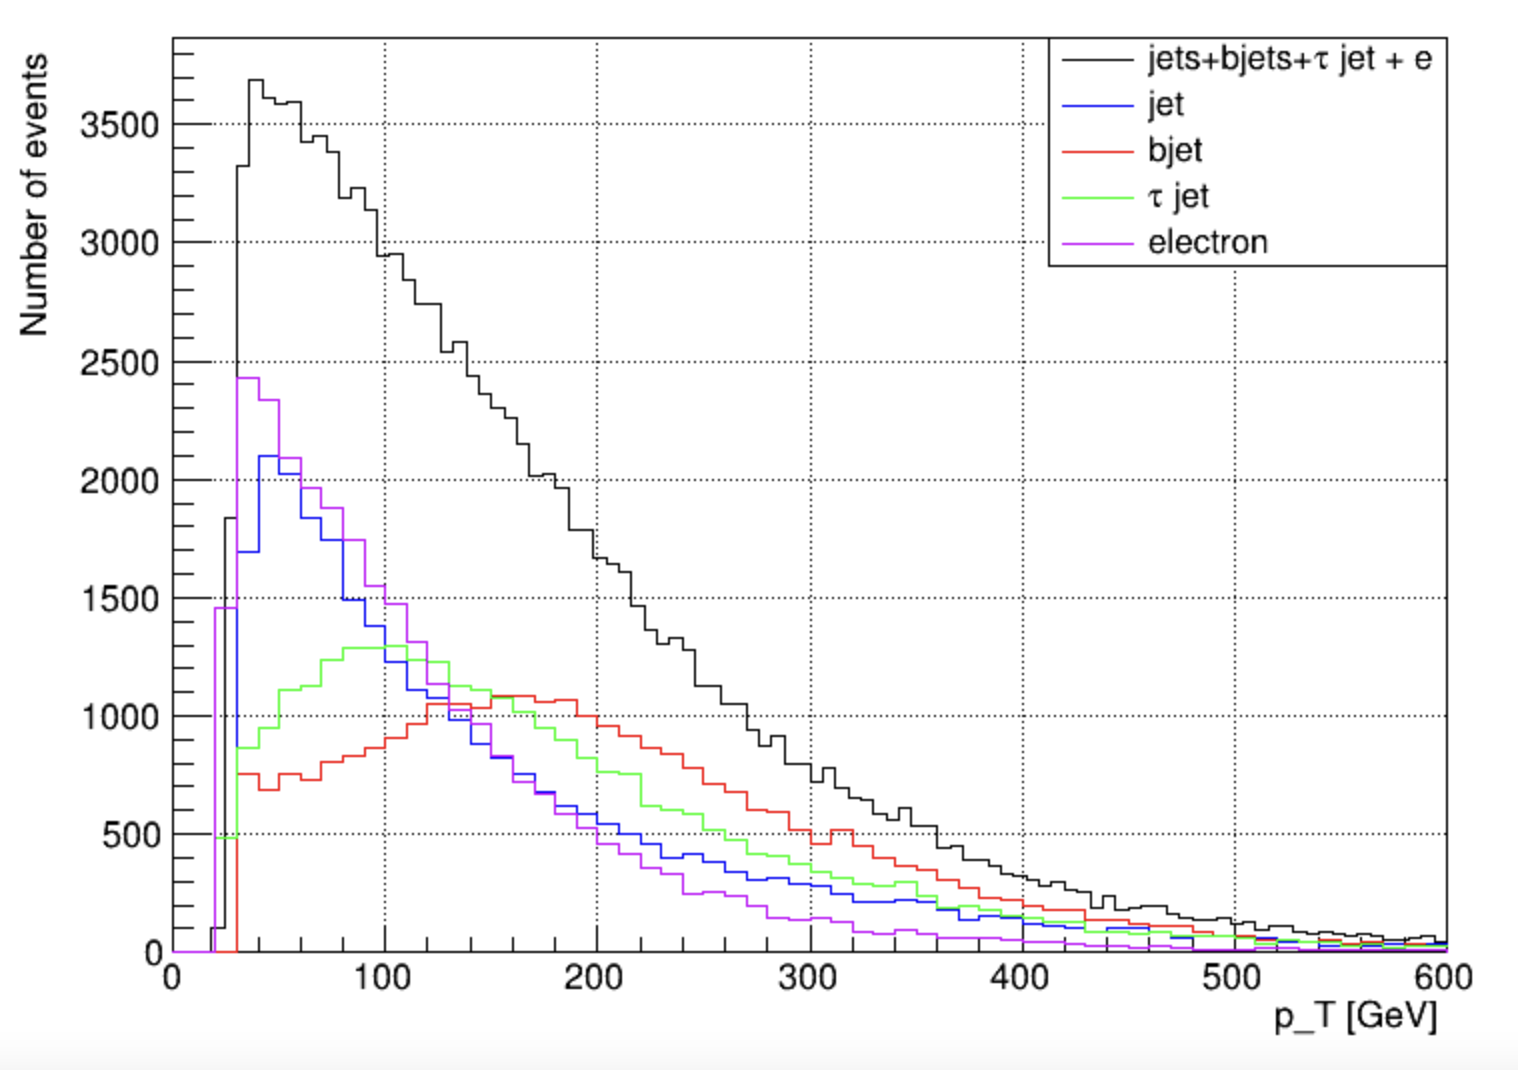
\includegraphics[width=\linewidth]{images/pt-electrons.png}
      \caption{Data for electronic decay}
      \label{fig:sub1}
    \end{subfigure}%
    \begin{subfigure}{.5\textwidth}
      \centering
      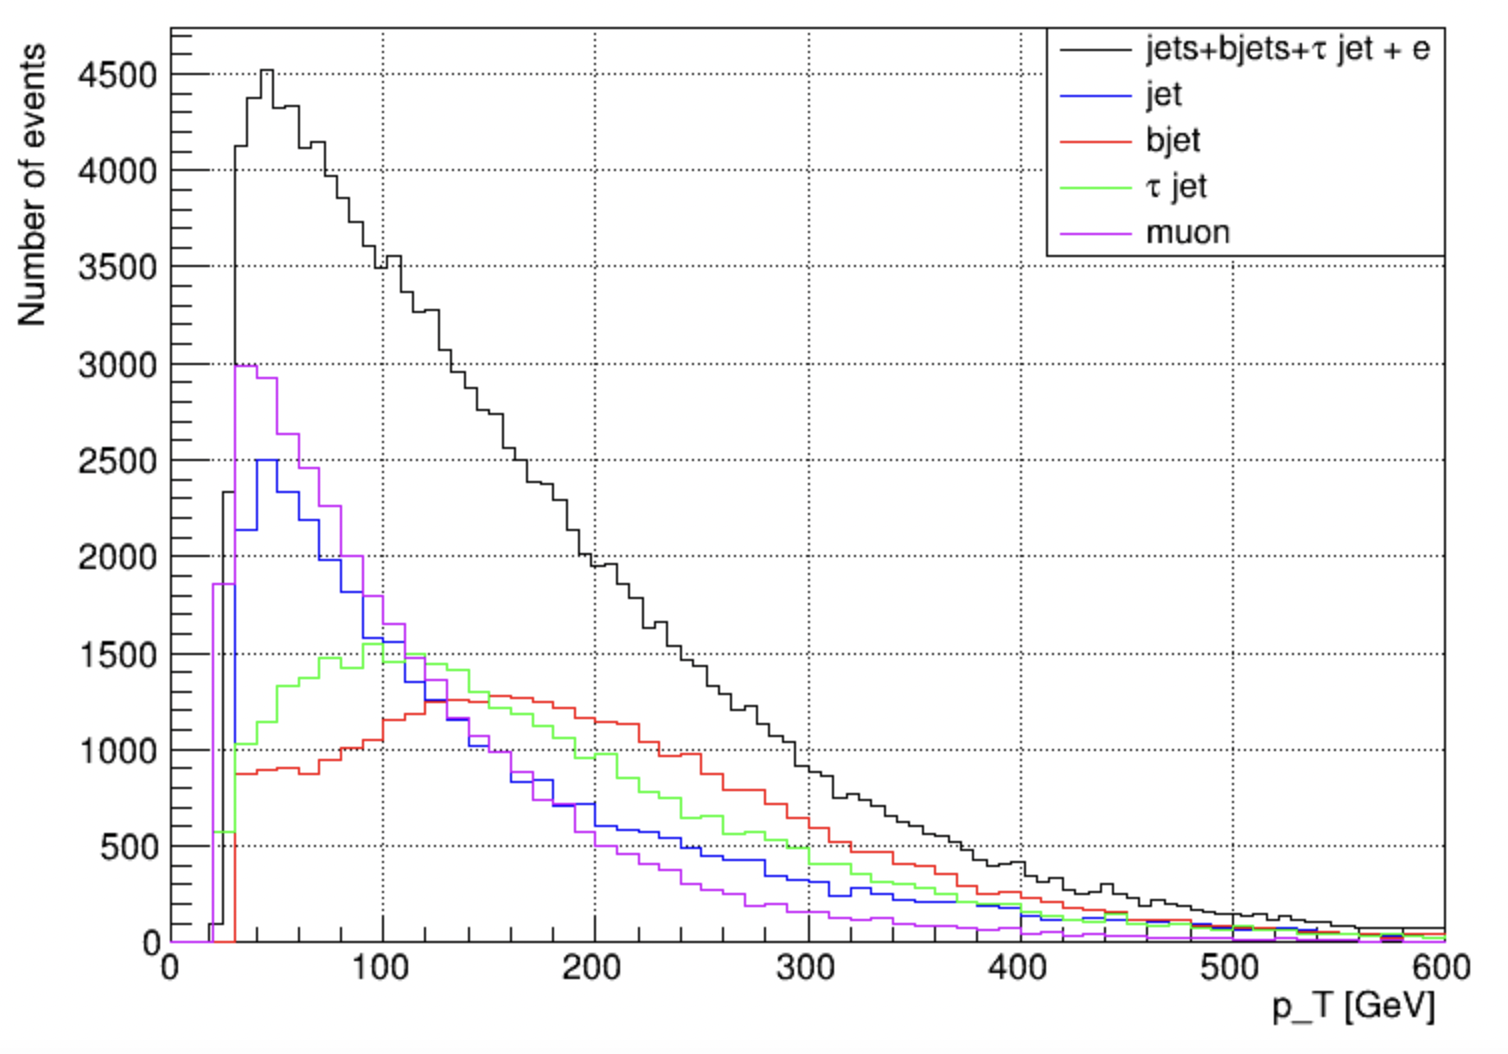
\includegraphics[width=\linewidth]{images/pt-muons.png}
      \caption{Data for muonic decay}
      \label{fig:sub2}
    \end{subfigure}
    \caption{Histograms showing the transverse momentum ($p_T$) for all jet types.}
    \label{fig:pT}
\end{figure}

The preliminary analysis concluded with the reconstructed mass for the leptoquark. Since the data does not provide information on which of the $\tau$'s decays leptonically and which decays hadronically, the reconstructed mass can be obtained by considering both decays. If the $\tau$ coming from the leptoquark decays leptonically, the leptoquark mass is the sum of the masses of the $b$-jet, the lepton and the missing transverse energy. If it decays hadronically, the reconstructed mass is just the sum of the $b$-jet and $\tau$-jet masses. The results for each decay mode are shown in figs. \ref{fig:recons_mass_e} and \ref{fig:recons_mass_mu}. Both in the decay to electrons and muons, the leptoquark mass is more efficiently reconstructed through leptonic decay than through hadronic decay. However, the distribution is wider in the former case due to the missing $E_T$ associated with the neutrinos.

\begin{figure}
    \centering
    \begin{subfigure}{.5\textwidth}
      \centering
      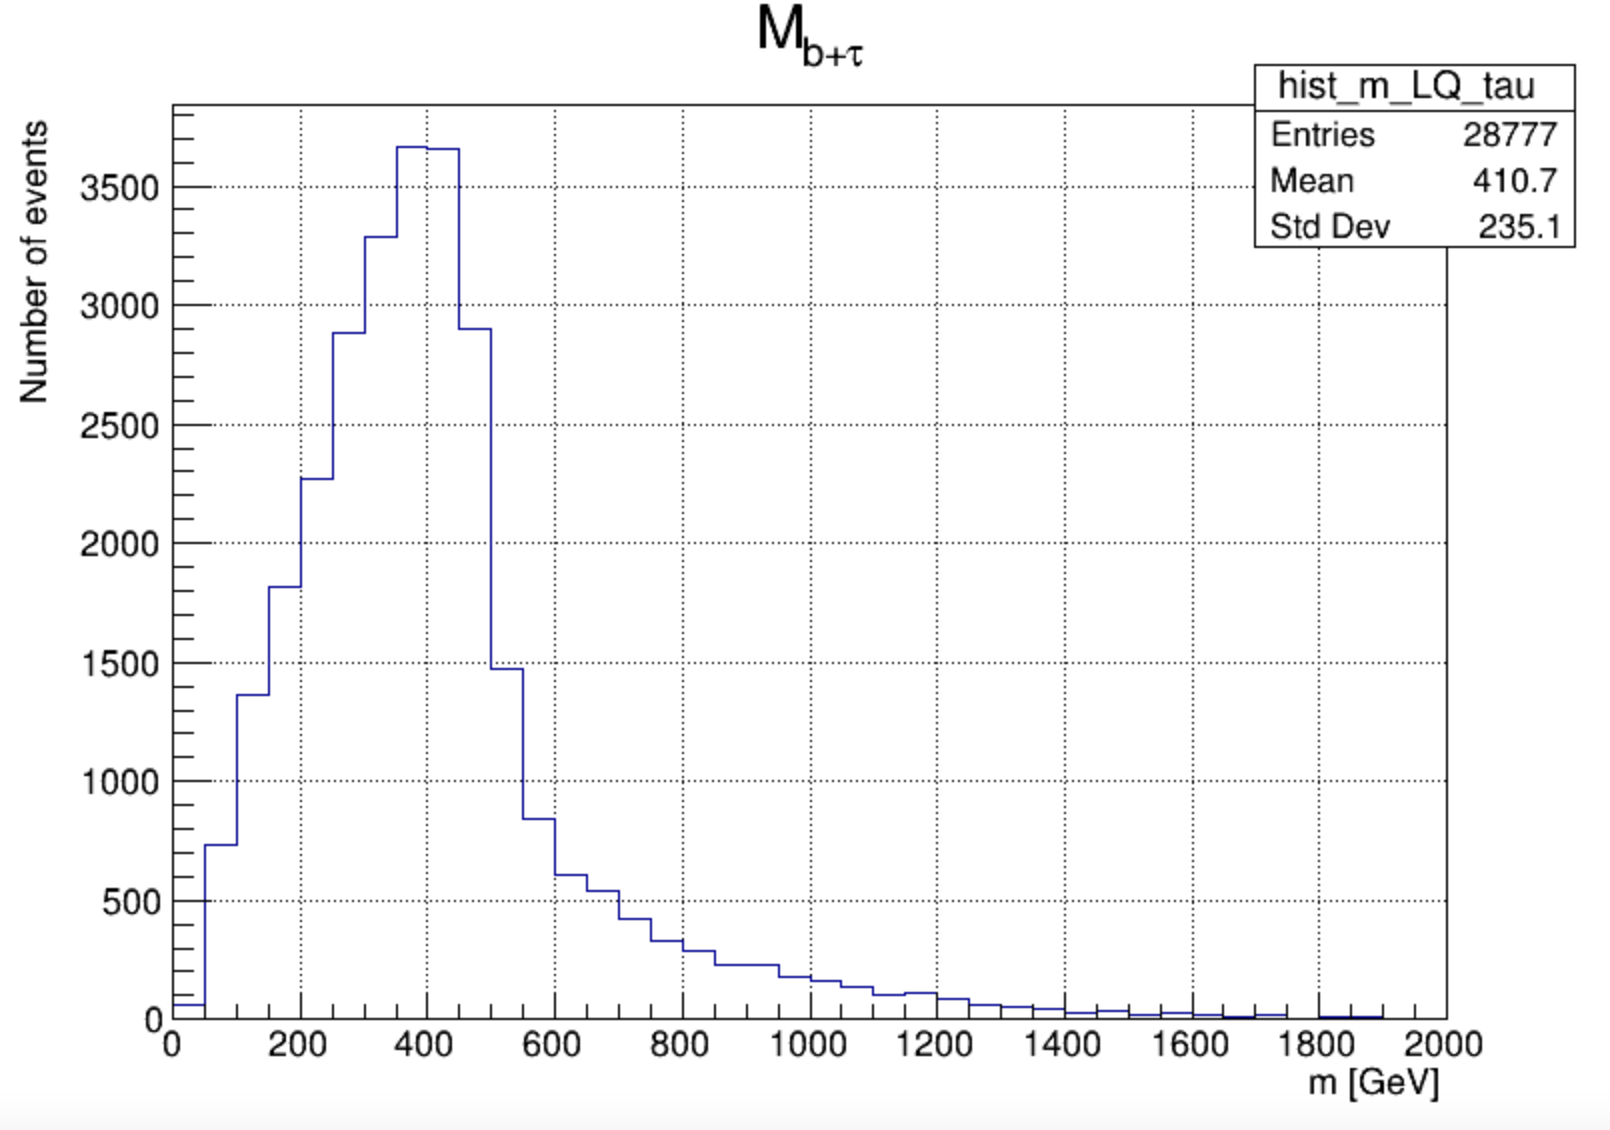
\includegraphics[width=\linewidth]{images/M-b_tau-electrons.png}
      \caption{}
      \label{fig:had-e}
    \end{subfigure}%
    \begin{subfigure}{.5\textwidth}
      \centering
      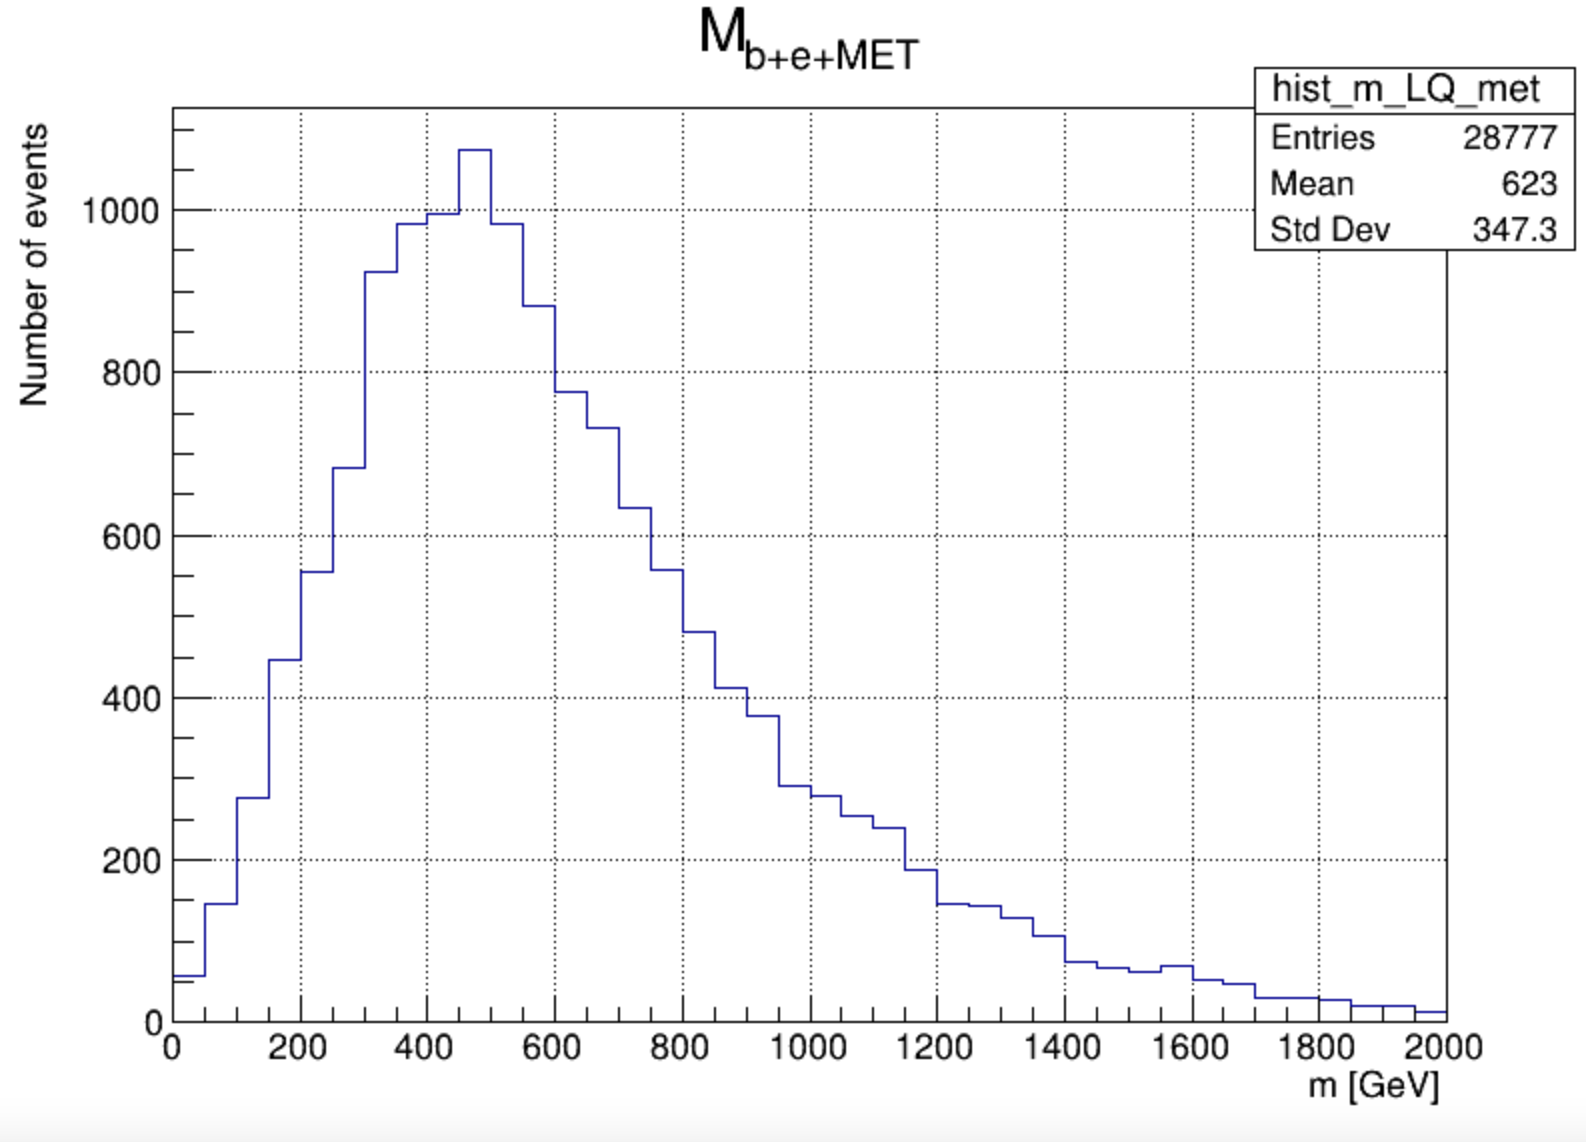
\includegraphics[width=\linewidth]{images/m-b_e.png}
      \caption{}
      \label{fig:lep-e}
    \end{subfigure}
    \caption{Histograms showing the reconstructed mass of the leptoquark assuming the $\tau$ lepton coming from the leptoquark decays hadronically (a) and leptonically to an electron-neutrino pair (b).}
    \label{fig:recons_mass_e}
\end{figure}

\begin{figure}
    \centering
    \begin{subfigure}{.5\textwidth}
      \centering
      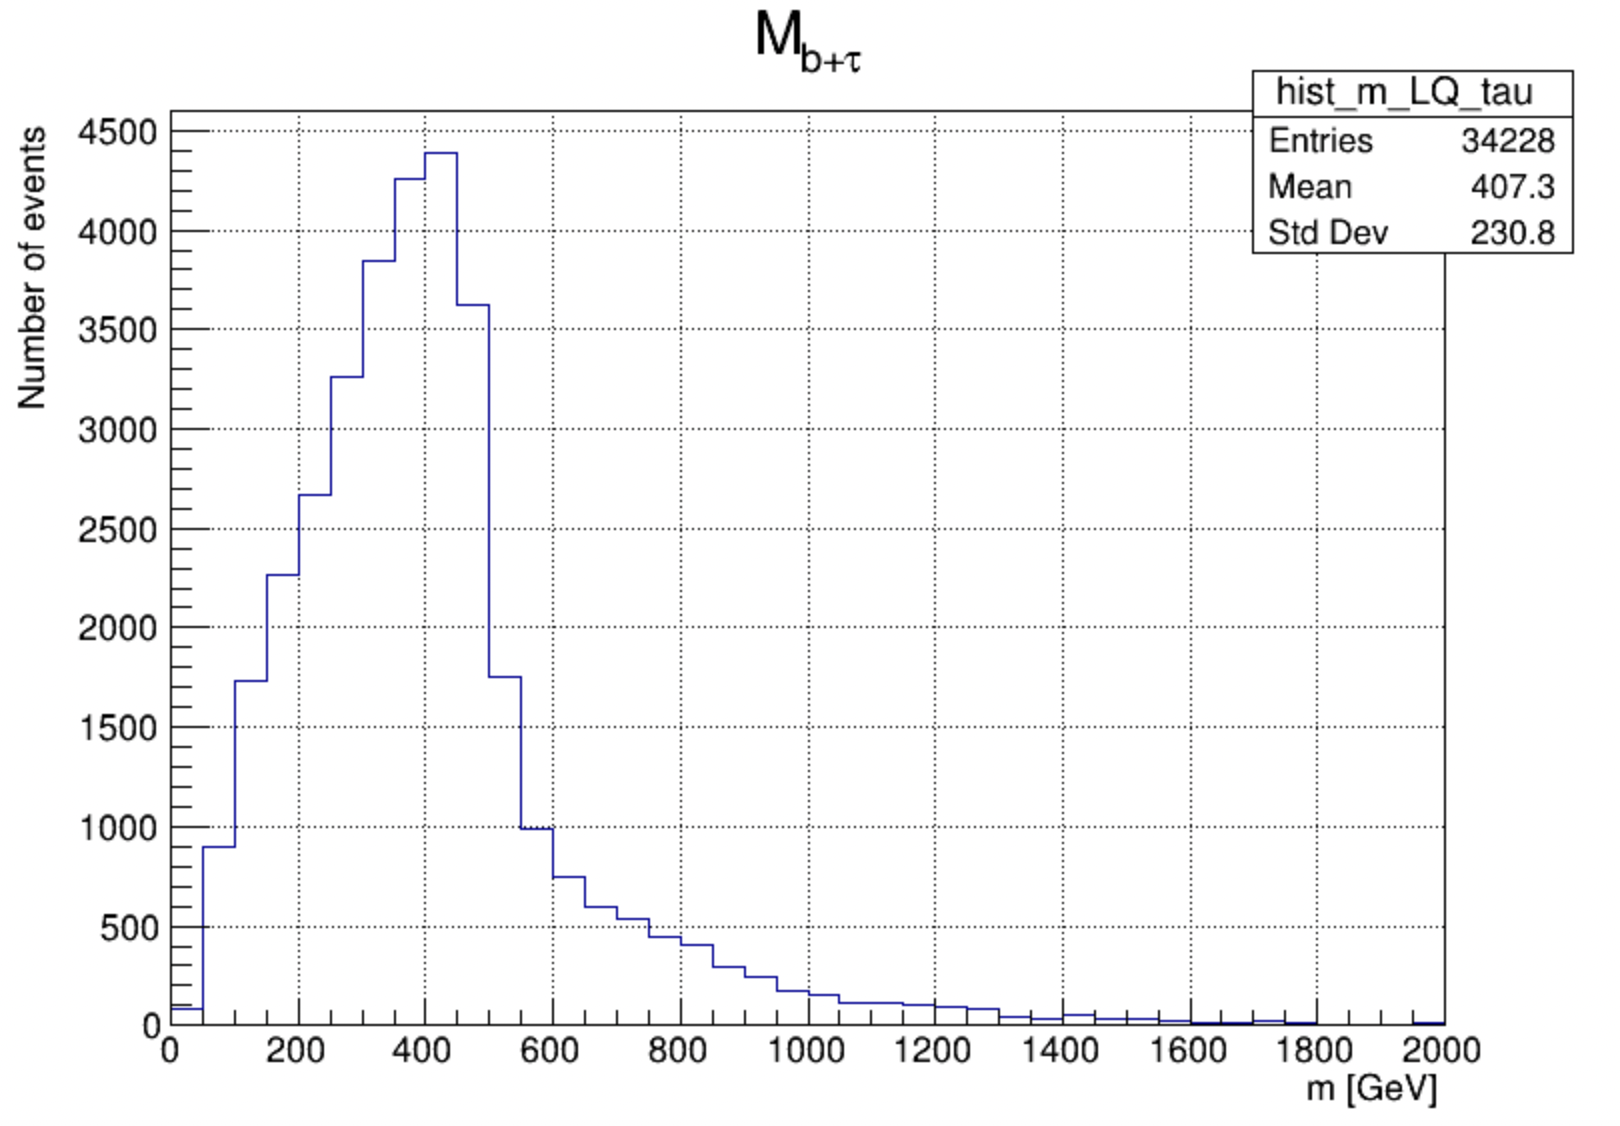
\includegraphics[width=\linewidth]{images/m-b_tau-muons.png}
      \caption{}
      \label{fig:had-mu}
    \end{subfigure}%
    \begin{subfigure}{.5\textwidth}
      \centering
      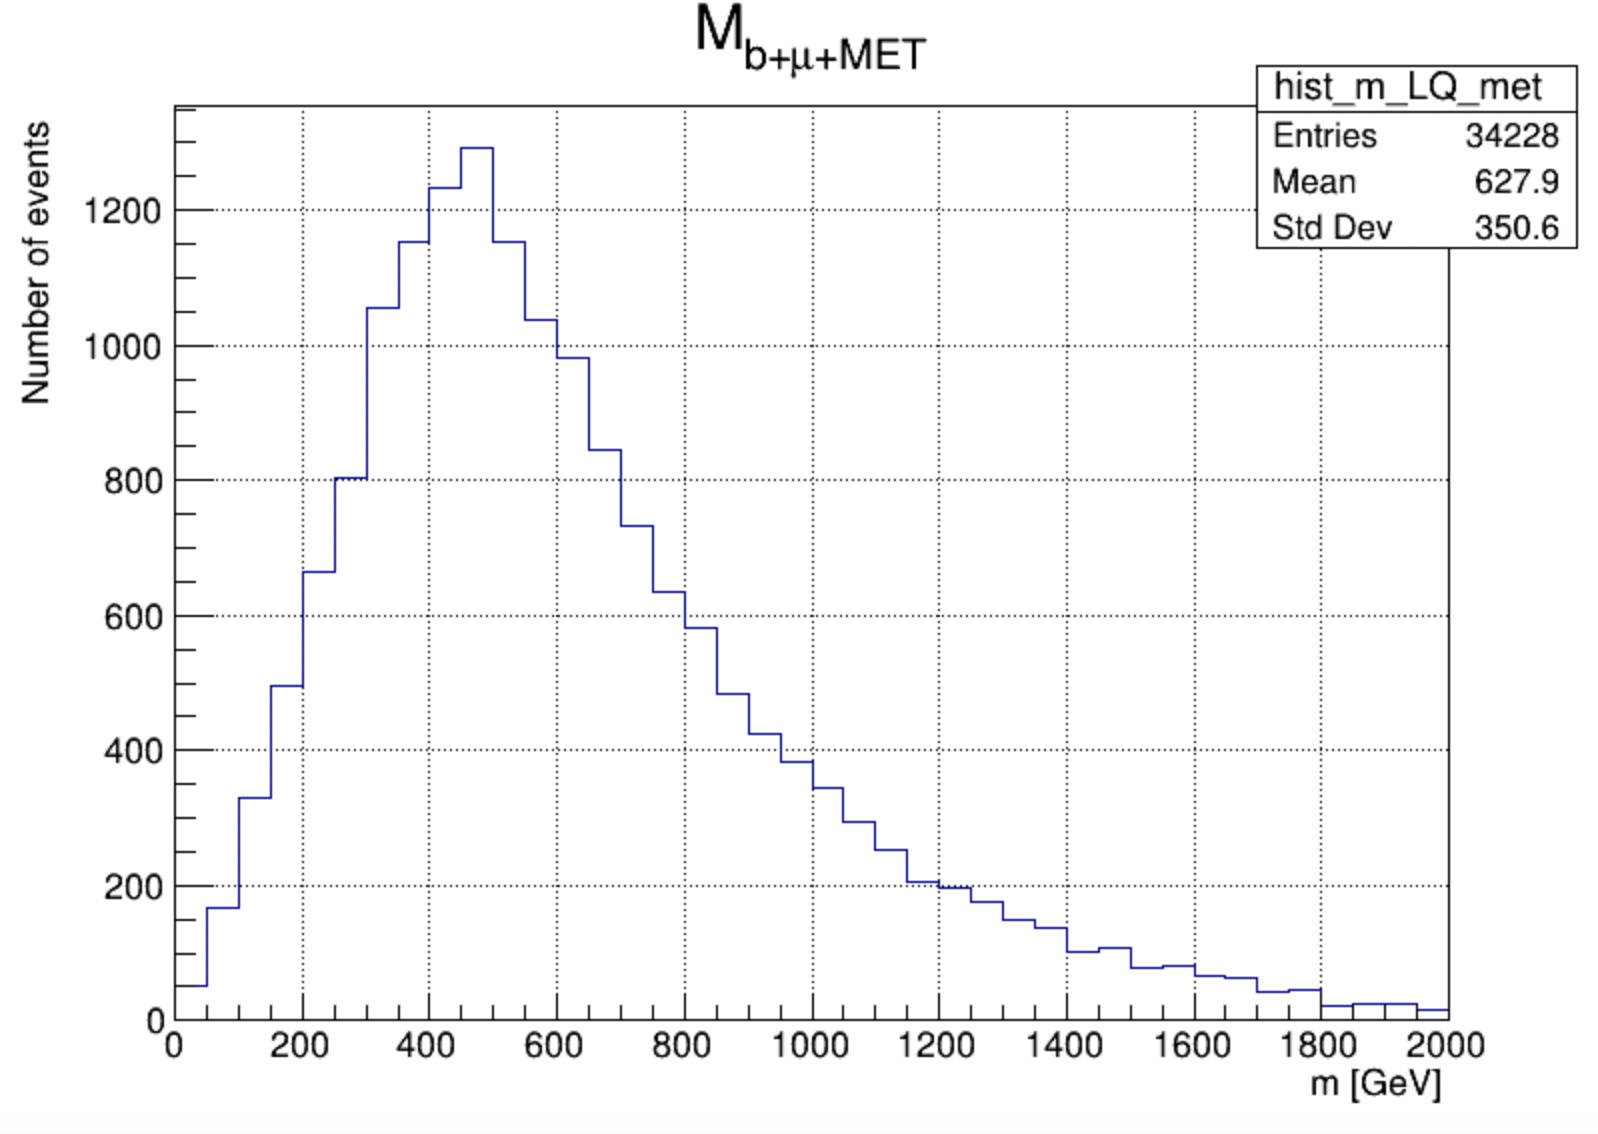
\includegraphics[width=\linewidth]{images/m-b_mu.png}
      \caption{}
      \label{fig:lep-mu}
    \end{subfigure}
    \caption{Histograms showing the reconstructed mass of the leptoquark assuming the $\tau$ lepton coming from the leptoquark decays hadronically (a) and leptonically to a muon-neutrino pair (b).}
    \label{fig:recons_mass_mu}
\end{figure}

Next steps in the analysis are: i) determine correlations between kinematical variables such as the pseudorapidity, the difference in momenta, and the azimuthal angle; ii) run the simulations with SM backgrounds; iii) examine the relationship between the production cross-section and model parameters such as leptoquark mass and coupling constant.


